\section{Behavior Results}
\label{sec:behave_result}
To understand how interfaces and options influenced survey response behaviors~(\textbf{RQ3}), we investigate time-to-action and remaining credit differences across experiment conditions. Time-to-action is a widely used metric in decision sciences, where longer decision time often indicates more complex cognitive processing~\cite{payneAdaptiveDecisionMaker1993}. Additionally, resource allocation strongly influences decision-making. \textcite{chengCanShowWhat2021} showed that the number of given credits influences the validity of QV. Decision science studies like \textcite{Shah2015a} and \cite{debruijnPovertyEconomicDecision2022} showed how scarcity influences decisions, increases risk aversion, and adds cognitive load. These measures serve as proxies for participant behavior, and all analyzed data is publicly available\footnote{link-to-github} for transparency and to facilitate further research.

\newsavebox{\savefig}

\begin{figure}[htbp]
    \centering
    \savebox{\savefig}{
        \begin{minipage}{0.7\pdfpageheight}
            \begin{subfigure}[b]{0.24\pdfpageheight}
                \centering
                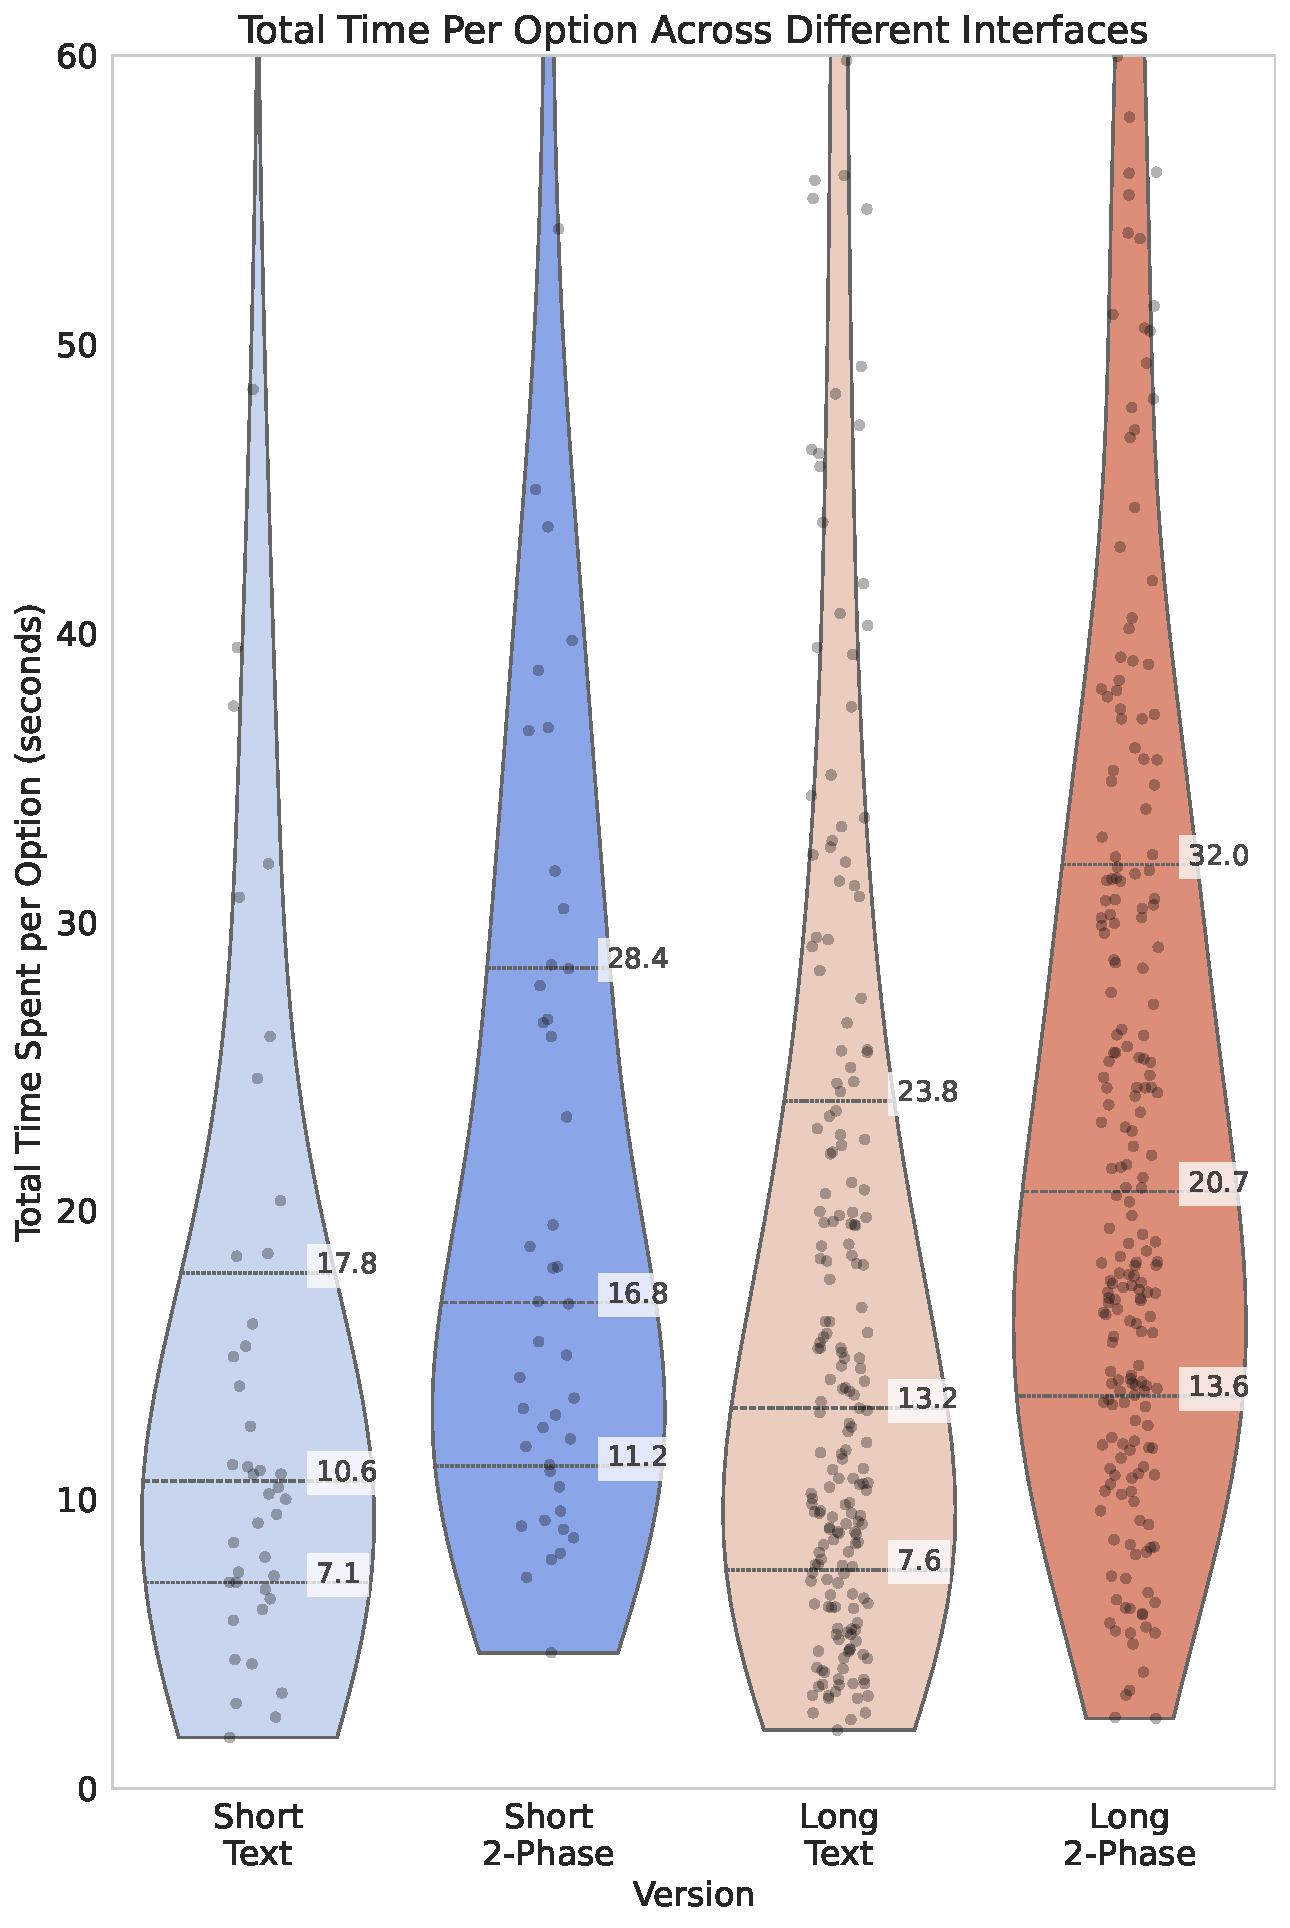
\includegraphics[width=\textwidth]{content/image/results/total_time_per_option.pdf}
                \captionsetup{width=0.87\textwidth}
                \caption{Total Time per option: We identified that the two-phase interface skewed slightly higher than the text interface, as expected. This discrepancy can be attributed to the extra organization step required in the two-phase interface, leading to a slightly longer overall completion time per option.}
                \Description{Violin plot showing total time spent per option in seconds across four interface versions: Short Text, Short 2-Phase, Long Text, and Long 2-Phase. The y-axis ranges from 0 to 60 seconds. Each violin plot has scattered dots representing individual data points. The shape of the Short Text plot is widest between 10 and 20 seconds, tapering at the top and bottom. The Short 2-Phase plot is the narrowest, with most dots concentrated between 10 and 20 seconds. The Long Text plot is narrow and widest near the bottom, between 5 and 15 seconds. The Long 2-Phase plot is widest near the top, between 20 and 40 seconds.}

                \label{fig:total_time}
            \end{subfigure}
            % \hfill
            \begin{subfigure}[b]{0.24\pdfpageheight}
                \centering
                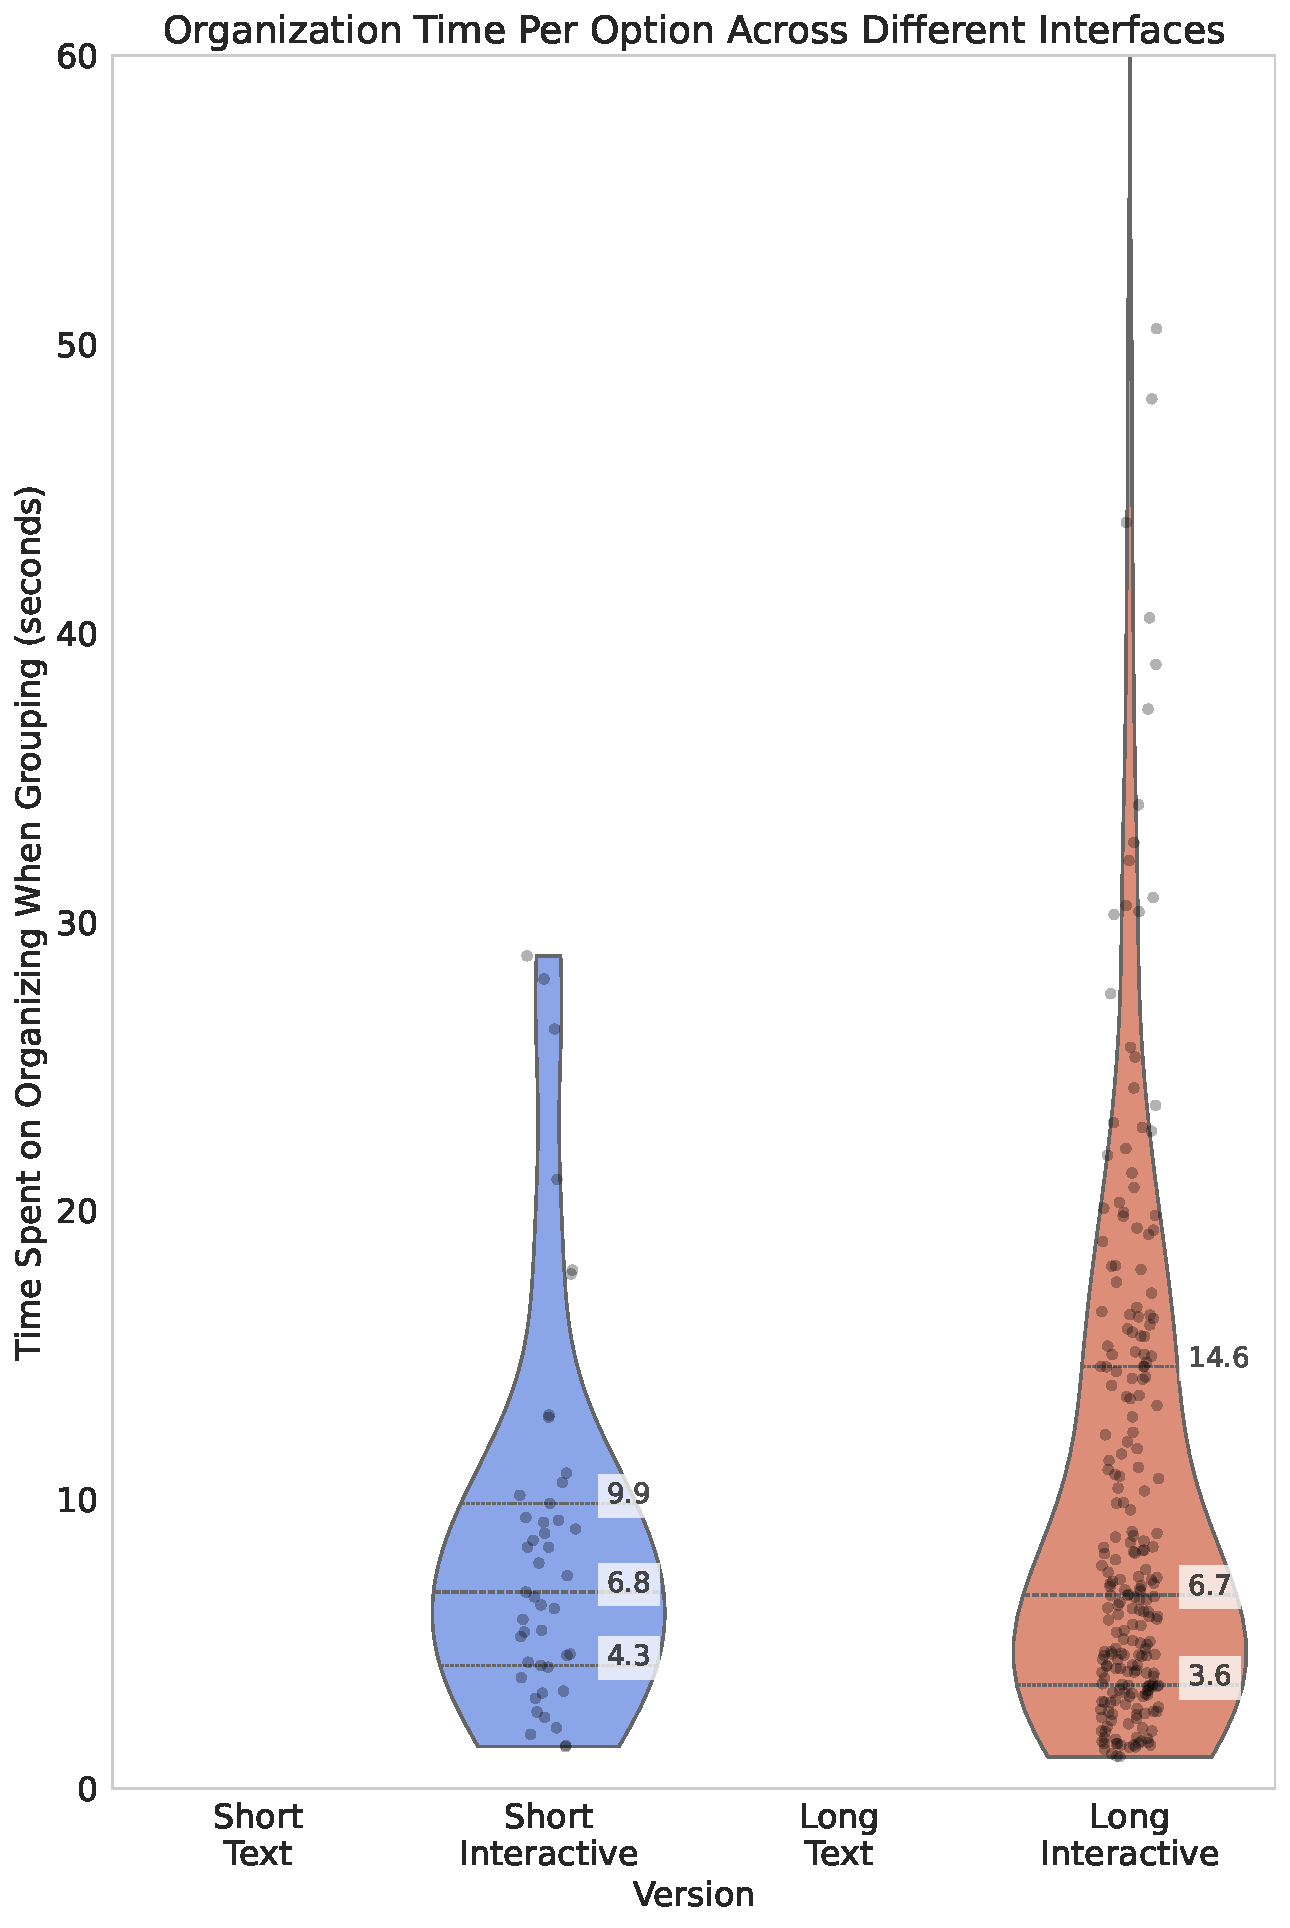
\includegraphics[width=\textwidth]{content/image/results/org_time_per_option.pdf}
                \captionsetup{width=0.87\textwidth}
                \caption{Organization Time per option: Only the two-phase interface includes an organization phase, hence the other experimental conditions do not exhibit any accumulated organization time. This figure reinforces that organization time was isolated to the two-phase design.}
                \Description{Violin plot showing time spent on organizing per option in seconds for two interface versions: Short 2-Phase and Long 2-Phase. The y-axis ranges from 0 to 60 seconds. The plot for Short 2-Phase is widest between 5 and 10 seconds, with scattered dots mostly concentrated between 4.3 and 9.9 seconds. The Long 2-Phase plot is narrower and taller, with most dots concentrated between 3.6 and 14.6 seconds, and a few outliers near the top. The Short 2-Phase plot has a rounded shape with a larger base, while the Long 2-Phase plot tapers sharply near the top.}

                \label{fig:org_time}
            \end{subfigure}
            % \hfill
            \begin{subfigure}[b]{0.24\pdfpageheight}
                \centering
                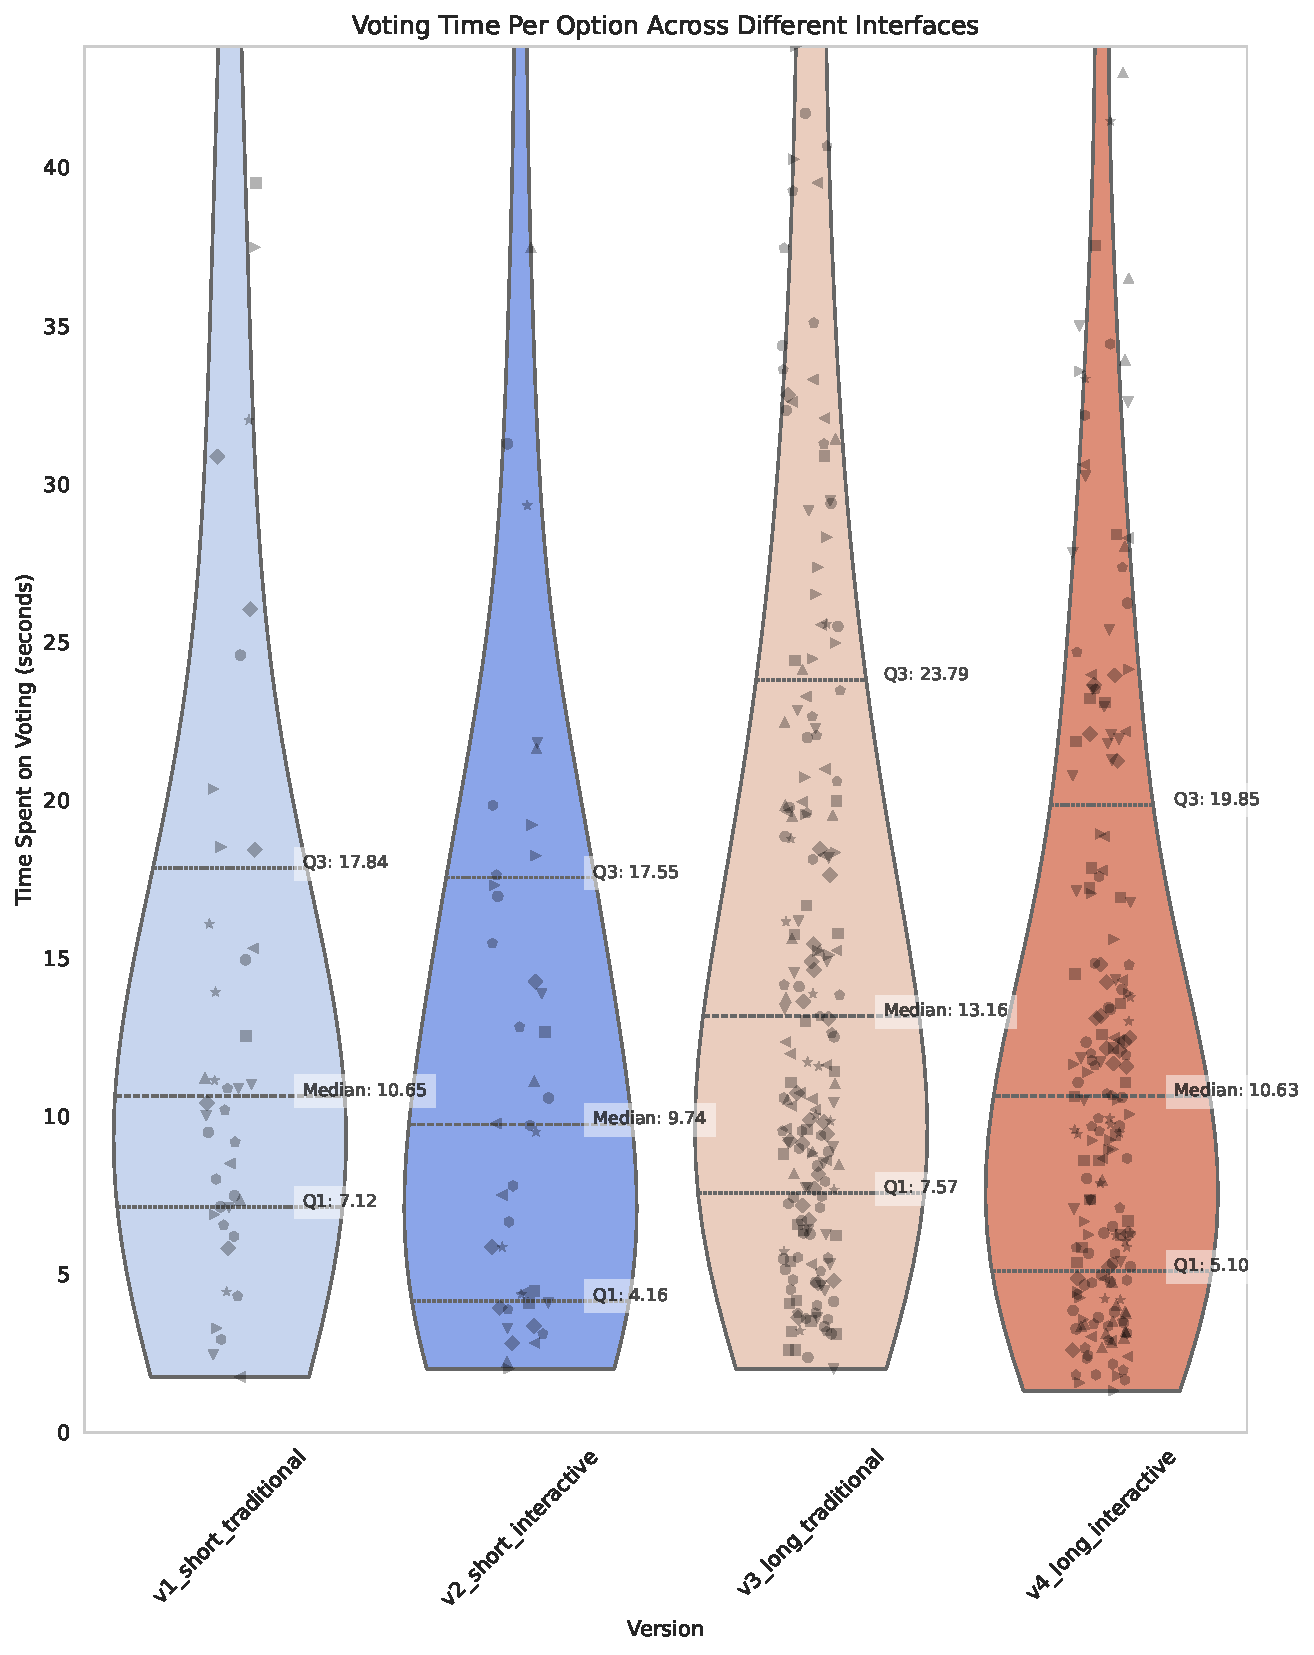
\includegraphics[width=\textwidth]{content/image/results/voting_time_per_option.pdf}
                \captionsetup{width=0.87\textwidth}
                \caption{Voting Time per option: We observe statistically significant faster voting times for the long QS in the two-phase interface. This suggests that the two-step design improves voting efficiency, especially for longer surveys.\vspace{1em}}
                \Description{Violin plot showing time spent on voting per option in seconds across four interface versions: Short Text, Short 2-Phase, Long Text, and Long 2-Phase. The y-axis ranges from 0 to 60 seconds. Each plot contains scattered dots representing individual data points. The Short Text plot is widest between 10 and 20 seconds, with most dots concentrated around 17.8 seconds. The Short 2-Phase plot has a narrow shape, with dots concentrated between 9.7 and 17.5 seconds. The Long Text plot is wider, with dots spread between 7.6 and 23.8 seconds. The Long 2-Phase plot has a wider shape near the top, with most dots between 10.6 and 19.8 seconds, and a few scattered near the top.}
                \label{fig:vote_time}
            \end{subfigure}
        \end{minipage}
    }
    \rotatebox{90}{%
        \begin{minipage}{\wd\savefig}
            
            \usebox{\savefig}
             \captionsetup{width=0.67\pdfpageheight}
            \caption{Time per option across all experiment conditions. The violin plots visualize time spent per option across the experimental conditions, with dots representing total time per option and horizontal lines indicating the median and interquartile ranges. While total time was slightly higher for the two-phase interface, the distinct phases (organization and voting) allowed for a more structured approach, particularly benefiting longer surveys.}
            \Description{A large figure containing three subfigures, all violin plots with scatterplots overlayed. From left to right, the subfigures are Time per option, organize time per option, and voting time per option across all experiment conditions }

            \label{fig:time_per_option_full}
        \end{minipage}
    }
\end{figure}


\subsection{Time Spent per Option}
\label{sec:time_per_option}
Our first analysis focuses on understanding how much time participants spent per option across different stages and experiment conditions. Based on the QS system log, we extracted the following detail:~\textit{the option}  involved in the interaction,~\textit{the type of interaction} (such as updating a certain number of votes), and~\textit{the time} between this interaction and the previous one. Each dot on Figure~\ref{fig:time_per_option_full} is a specific type of time a participant spent for one option. 

\paragraph{Total time} Total time is the aggregate of all time spent on each option across both phases. Each dot on Figure~\ref{fig:total_time} visualizes the total time. Participants spent slightly more time per option on the two-phase interface than the text interface. A non-parametric Mann-Whitney U test showed a small effect size (long QS: $p<0.0000001$, Rank-biserial: $-0.304$, Cohen's d: $0.030$; short QS: $p=0.01$, Rank-biserial: $-0.37$, Cohen's d: $0.082$). This is expected as the two-phase interface has an additional step of organizing the options. 

We further break down the total time spent into organization time and voting time. To minimize noise, we intentionally dropped all the time participants spent on the first option in the organization phase or voting phase. The goal is to exclude time spent on reading the prompt, forming their preference, or understanding the interface.

\paragraph{Organization time} Organization time covers both placing options into categories and the drag-and-drop time during the organization phase. Illustrated in Figure~\ref{fig:org_time}, we observed minimal difference in organization time per option between short and long surveys, as the interface shows options one at a time for categorization. It also suggests that even for longer surveys, the organization functionalities did not significantly impact the time participants needed for an option.

\paragraph{Voting time} Voting time strictly refers to the time participants took to update vote values for each option. As shown in Figure~\ref{fig:vote_time}, participants spent significantly less time voting on the two-phase interface than on the text interface with a small effect size in the long QS ($U=24053$, $p<0.005$, Rank-biserial: $0.167$, Cohen's d: $0.017$), but not in the short survey ($p>0.4$, Power=$0.051$). This supports our hypothesis that the two-step design in the two-phase interface facilitates more efficient decision-making, especially in longer surveys.

\begin{figure}[h]
    \centering
    \begin{subfigure}[b]{\textwidth}
        \centering
        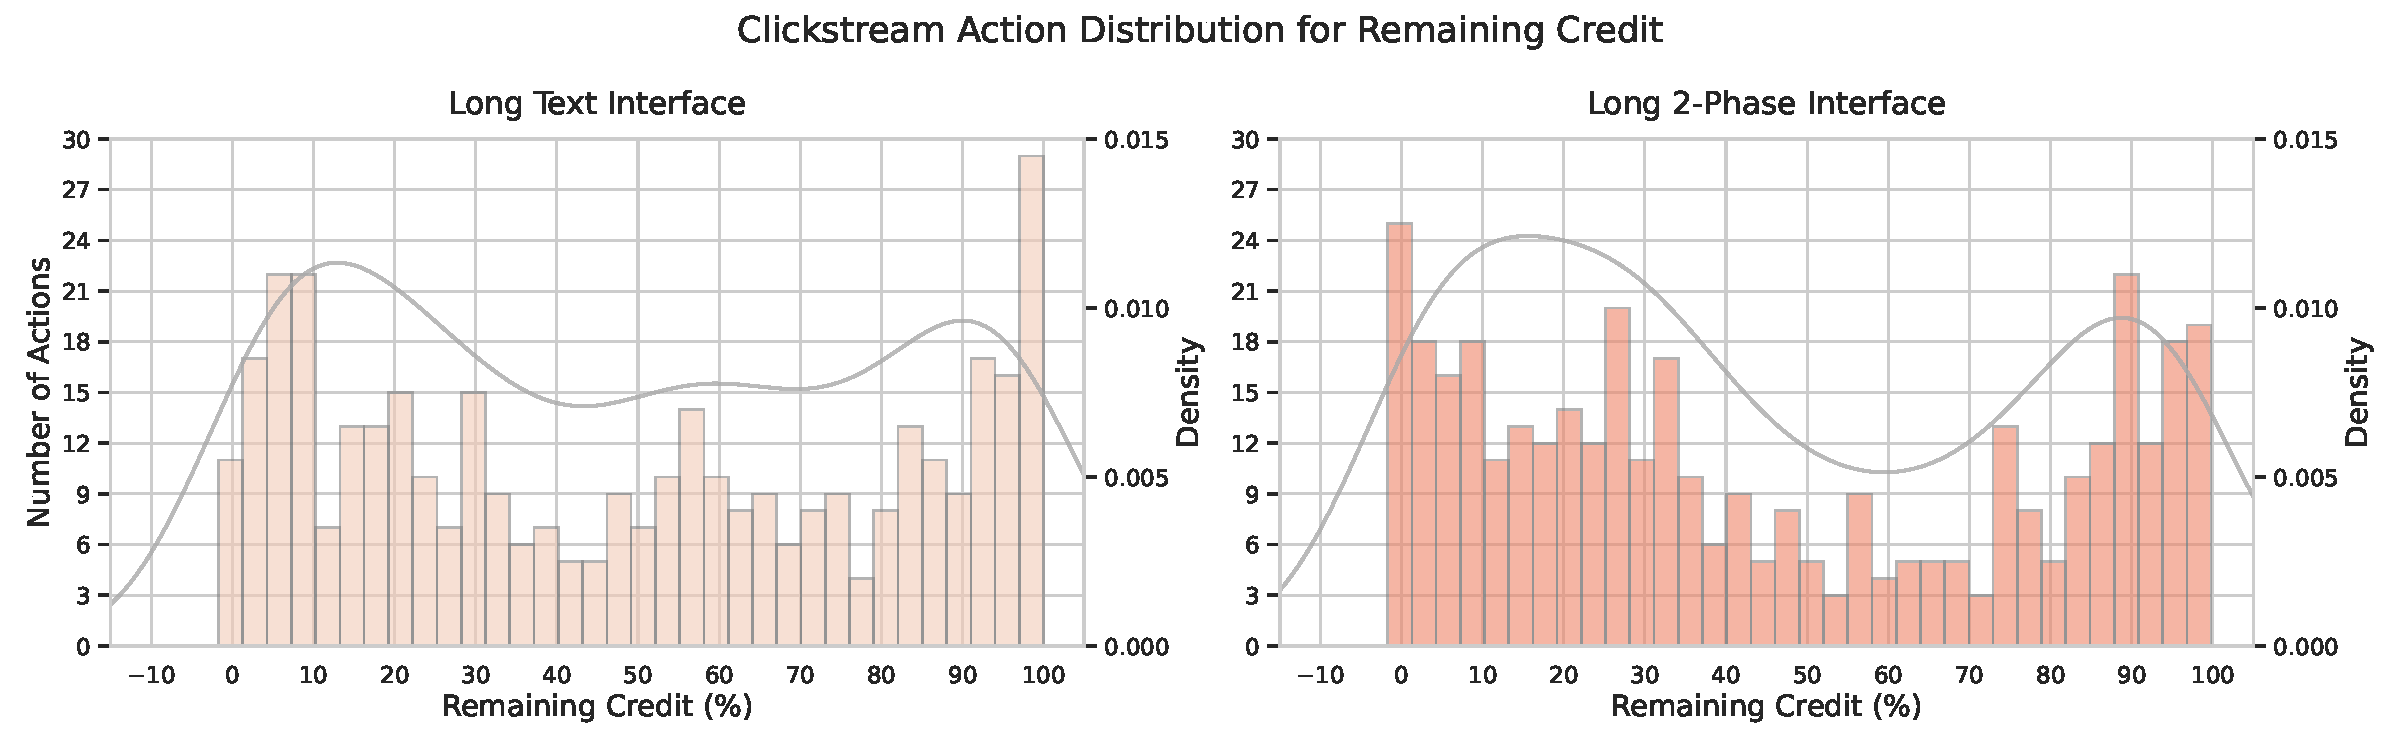
\includegraphics[width=\textwidth]{content/image/results/new_clickstream_action_distribution_lower_row.pdf}
        \caption{This plot counts the number of voting actions when there are $x$ percentages of credits remaining. A KDE plot is provided to help better understand the action distribution.}
        \Description{A dual-panel histogram with overlaid KDE curves showing the distribution of voting actions based on remaining credit percentages for two interfaces: Long Text and Long 2-Phase. The x-axis shows the remaining credit as a percentage, ranging from -10\% to 100\%, and the y-axis on the right shows density for the KDE curves. In the left panel for the Long Text interface, the KDE curve rises sharply to a peak around 10\%, gradually declines, and then rises again toward 100\%, with a moderate dip in the middle. In the right panel for the Long 2-Phase interface, the KDE curve shows more pronounced changes: it rises steadily from 10\% to 30\%, then dips more sharply than the left panel, before rising to a prominent peak near 100\%. The right curve has a deeper dip and a broader rise compared to the left.}
        \label{fig:all_clicks}
    \end{subfigure}
    
    \vspace{1em} % Adjusts the space between the subplots
    
    \begin{subfigure}[b]{\textwidth}
        \centering
        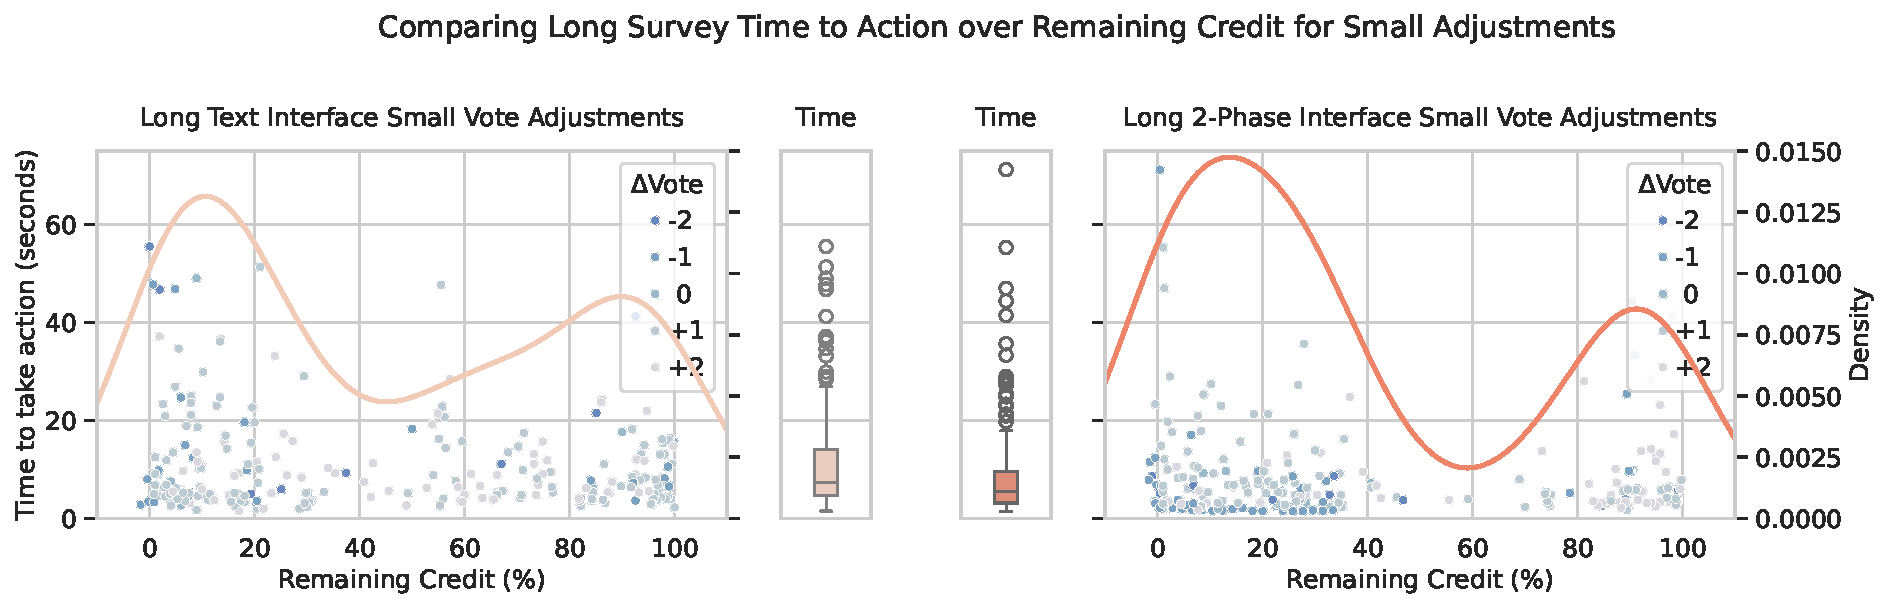
\includegraphics[width=\textwidth]{content/image/results/small_adjustments_plot.pdf}
        \caption{This plot further separates participants' interaction behavior based on the number of votes participants adjusted. We observed a bimodal interaction pattern across long QS when small vote adjustments are made.}
        \Description{A dual-panel plot comparing time to take action in seconds over remaining credit percentages for small vote adjustments in two interfaces: Long Text and Long 2-Phase. The x-axis shows remaining credit as a percentage, from 0\% to 100\%, and the y-axis on the left shows the time to take action in seconds, ranging from 0 to 60. Both panels feature scatter plots with colored dots representing vote changes from -2 to +2. The left panel shows the Long Text interface, with an orange density line rising sharply, peaking around 20\% remaining credit, then dipping around 50\%, and rising again near 100\%. The right panel shows the Long 2-Phase interface with a similar pattern, but the peaks and dips are more pronounced, especially with a sharper dip near 50\%. A box plot on the far right summarizes action time, showing the spread and median time for each interface.}

        \label{fig:small_clicks}
    \end{subfigure}
    
    \caption{Comparison of voting actions and participant behavior in different survey interfaces. Subplot (a) shows the overall distribution of actions based on the remaining credit, while subplot (b) further differentiates the interaction based on the size of vote adjustments.}
    \label{fig:combined_voting_behavior}
\end{figure}


\subsection{Budget and Voting Behaviors}
We further breakdown and highlight key differences of how long QS participant's voting behaviors when credits changed their voting behaviors with detailed analysis in Appendix~\ref{apdx:additional_results_behavior}. Figure~\ref{fig:all_clicks} first shows the number of vote adjustments at a given remaining budget across the two interfaces. We then plotted the vote adjustments of two or fewer votes, which is $10\%$ of the possible values one can choose among the maximum of 21 votes in Figure~\ref{fig:small_clicks}. A kernel density estimate (KDE) plot is provided to visualize the trends and compare how it changed when we plotted only small vote adjustments.

In long surveys, participants exhibited more actions both when the budget was abundant and when it began to run out. This pattern was more pronounced with the long two-phase interface. In fact, the bimodal distribution is more pronounced in the two-phase interface. This suggests that participants make small adjustments both at the beginning and toward the end of the QS. However, the two-phase interface shows more frequent and faster edits towards the end. Visually, dots are more clustered in the long two-phase interface for small vote adjustments compared to the long text interface. The Mann-Whitney U Test on the time spent on small vote adjustments showed significant differences ($U=13037$, $p<0.001$), with a small effect size (Rank-biserial: $0.227$, Cohen's d: $0.195$) and a power of $0.381$. This indicates that participants had a clearer idea of how to distribute their credits across the options.

Five participants highlighted how the interface supported their incremental iterative approach during the interview whom all used the two-phase interface. As one participant pointed out:

\begin{displayquote}
I like the fact that it remembers everything that you know.~\bracketellipsis that's very important is that it's an iterative process.\hfill\quoteby{S019 (LI)}
\end{displayquote}

\textbf{In summary}, participants spent more time on the two-phase interface compared to the text interface in both short and long surveys. Across the two-phase interfaces, organization time remained consistent. While voting time did not differ between interfaces for the short survey, participants voted more quickly on the two-phase interface in the long survey, confirming the hypothesis that the two-step design enhances decision-making efficiency. Voting behaviors indicated more frequent actions when the budget was abundant and nearly exhausted, particularly in the long two-phase interface. Additionally, the analysis revealed more frequent and faster small vote adjustments towards the end of the QS in the two-phase interface, demonstrating an iterative and incremental approach. 

% content removed in discussion should make sure are in this section
%  , as reflected in slightly faster voting times

% This suggests that participants in the interactive interface are more likely to make larger adjustments to their votes. This is consistent with the observation that participants in the interactive interface spent more time on voting actions in the long survey. We also see a cluster of voting actions in the bottom left corner of the interactive interface for small vote adjustments. This suggests that participants in the interactive interface are more likely to make small adjustments when their budget is running low. This is consistent with the observation that participants in the interactive interface spent less time on voting actions in the long survey.
% First, surface the bimodal action distribution in both plots, with a even stronger signal for long interactive interface participants. Second, the plot demonstrated a clear cluster of voting actions in the bottom left corner of the interactive interface for small vote adjustments. In other words, participants made much smaller but more rapid adjustments when their budgets were running low. Second, larger adjustments are made when the participants have more options comparing the two plots on the first row. We interpret this behavior as participants in the interactive interface have constructed a clearer image of option preferences and, hence, have the ability to take larger strides in allotting their budget and deciding the number of votes at the beginning of the survey. Toward the end, participants using the interactive interface are then making fine-tuned adjustments to ensure that their preferences are reflected in their submissions.

% add qualitative support


% Ti-Chung Cheng: So what elements of the software interface do you dislike, or like the most, if any, when expressing your preferences on responding to societal issues?
% S009: Hmm! What I like the most actually, probably the sorting function. I think that it really helped me organize my thoughts really, clearly, in terms of what I would dislike the most. really, not that much. I would say. yeah, also, like how we could categorize it, like even within the voting stage rather than just at the categorization stage. 

% Ti-Chung Cheng: Can you tell me a little bit more about the screen? How did the vertical screen help you?
% S037: I think because it helps the layout of, because it's like a long 3 bar. So it's easier for you to to drag and drop, and you can actually sort it, judging by the votes. But I do not do that. But I think this layout is could be helpful in that aspect.


